\documentclass{article}
\usepackage[margin=1cm]{geometry}
\usepackage{fp}
\usepackage{siunitx}
\usepackage{tikz}

\begin{document}
\begin{center}
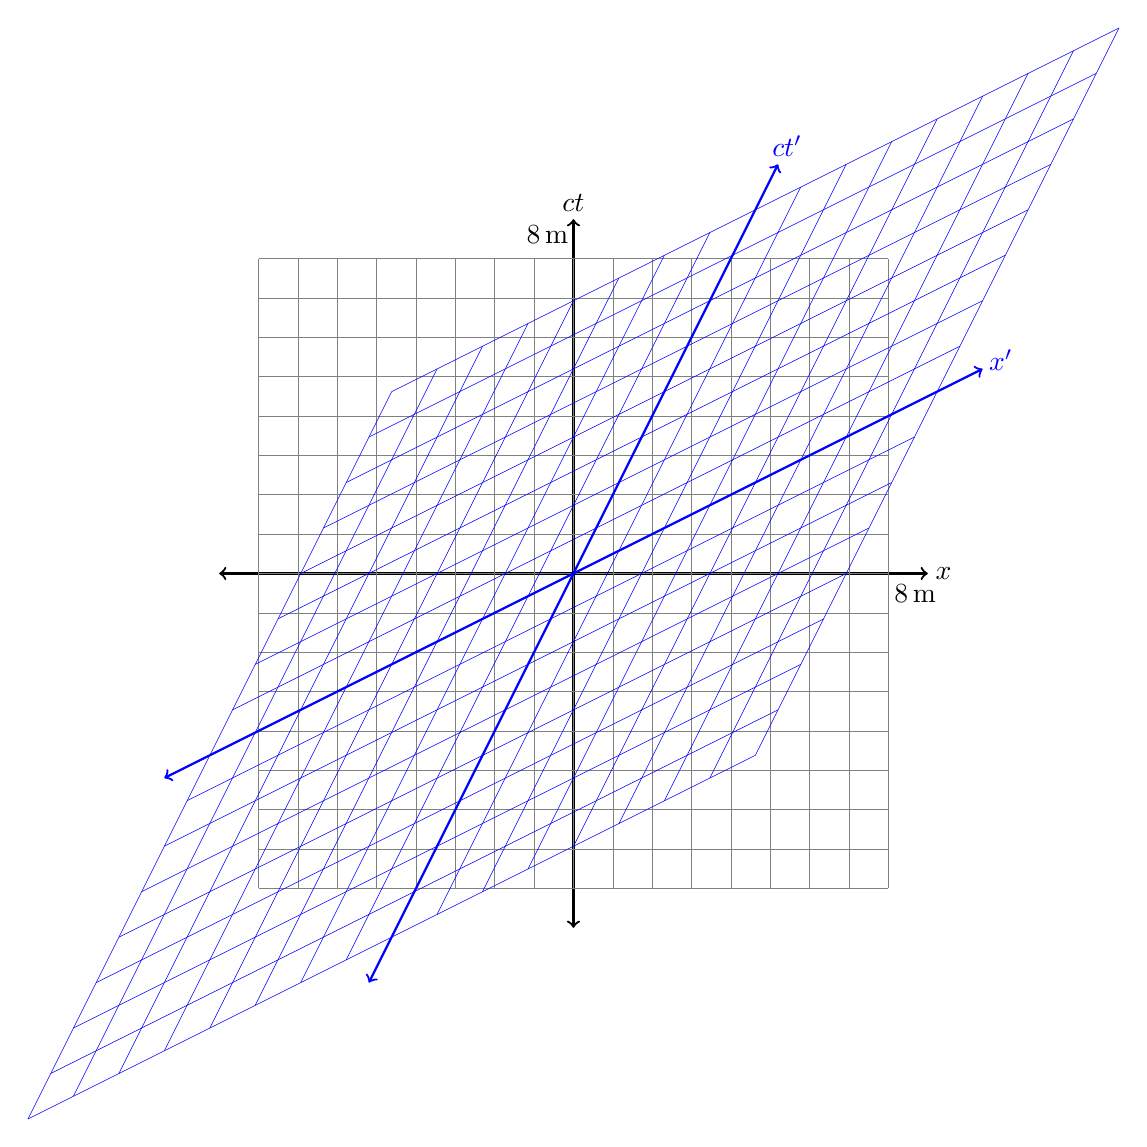
\begin{tikzpicture}

% This command generates a Minkowski space diagram.
% 
% Parameter 1: width of 1 grid space
% Parameter 2: maximum x/ct value
% Parameter 3: proportion of speed of light
\newcommand{\spacetimediagram}[3]{
    % Draw the x and ct axes
    \draw[<->,thick] (-#2*#1-#1, 0) -- (#2*#1+#1, 0);
    \draw[<->,thick] (0, -#2*#1-#1) -- (0, #2*#1+#1);
    % Draw the x ct grid
    \draw[step=#1,gray,very thin] (-#2*#1, -#2*#1) grid (#2*#1, #2*#1);

    % Evaluate the Lorentz transformation
    \FPeval{\calcgamma}{1/((1-(#3)^2)^.5)}
    \FPeval{\calcbetagamma}{\calcgamma*#3}

    % Draw the x' and ct' axes
    \draw[<->,thick,cm={\calcgamma,\calcbetagamma,\calcbetagamma,\calcgamma,(0,0)},blue] (-#2*#1-#1, 0) -- (#2*#1+#1, 0);
    \draw[<->,thick,cm={\calcgamma,\calcbetagamma,\calcbetagamma,\calcgamma,(0,0)},blue] (0, -#2*#1-#1) -- (0, #2*#1+#1);

    % Draw the vertical transformed grid lines
    \foreach \x in {-#2,...,#2}
        \draw[cm={\calcgamma,\calcbetagamma,\calcbetagamma,\calcgamma,(0,0)},blue,very thin] (\x*#1,-#2*#1) -- (\x*#1,#2*#1);
    % Draw the horizontal transformed grid lines
    \foreach \y in {-#2,...,#2}
        \draw[cm={\calcgamma,\calcbetagamma,\calcbetagamma,\calcgamma,(0,0)},blue,very thin] (-#2*#1,\y*#1) -- (#2*#1,\y*#1);

    % Draw the x and ct axes labels
    \draw (#2*#1+#1+0.2,0) node {$x$};
    \draw (0,#2*#1+#1+0.2) node {$ct$};
    % Draw the x' and ct' axes labels
    \draw[cm={\calcgamma,\calcbetagamma,\calcbetagamma,\calcgamma,(0,0)},blue] (#2*#1+#1+0.2,0) node {$x^\prime$};
    \draw[cm={\calcgamma,\calcbetagamma,\calcbetagamma,\calcgamma,(0,0)},blue] (0,#2*#1+#1+0.2) node {$ct^\prime$};
    
    % Draw the unit indicators
    \draw (#2*#1+0.34,-0.26) node {$\qty{#2}{\m}$};
    \draw (-0.33,#2*#1+0.3) node {$\qty{#2}{\m}$};
}

% Generate the spacetime diagram with a given grid spacing, grid count, and beta value:
% Modify these values to change the diagram's characteristics.
\spacetimediagram{.5}{8}{1/2}

\end{tikzpicture}
\end{center}
\end{document}